\documentclass[tikz,border=3pt,11pt]{standalone}
\usepackage[utf8]{inputenc}
\usepackage[T1]{fontenc}
\usepackage[brazilian]{babel}
\usepackage{tikz}
\usetikzlibrary{arrows.meta,positioning,calc}
\renewcommand{\familydefault}{\sfdefault}
\definecolor{ink}{HTML}{202124}
\definecolor{muted}{HTML}{666666}
\definecolor{blue}{RGB}{30,80,160}
\definecolor{green}{RGB}{30,130,60}
\definecolor{red}{RGB}{190,60,60}
\definecolor{light}{HTML}{E8E8E8}
\tikzset{flow/.style={-{Stealth[length=2.5mm]},line width=1pt,draw=blue},
  label/.style={font=\normalsize,text=ink,align=center},
  stop/.style={circle,minimum size=9mm,inner sep=0pt,line width=1pt,font=\bfseries},
  every node/.style={text=ink}}

\usepackage{alltt}
% Fluxo do compilador de regras: interface -> TOML -> compilador -> planejador,
% com um exemplo de cada passo (a regra da higienizacao, em
% projeto-inovacao-grupoB/exemplos/sinteticas-ciclo2.toml). Os exemplos ficam
% em duas alturas intercaladas, para poderem ser maiores. Os trechos de texto
% sao reais e terminam em "..." onde foram cortados.
\newsavebox{\toml}
\newsavebox{\pddl}
\begin{lrbox}{\toml}\begin{minipage}{2.95cm}\fontsize{5}{6}\selectfont
\begin{alltt}
[[preparo]]
nome = "higienizar-maos"
estado = "maos-higienizadas"
consome = "alcool"
custo = 2
desfeito_ao_sair = true
exigido_antes_de = [
  "pressao", "glicemia", ...]
\end{alltt}
\end{minipage}\end{lrbox}
\begin{lrbox}{\pddl}\begin{minipage}{3.2cm}\fontsize{5}{6}\selectfont
\begin{alltt}
(:action higienizar-maos
  :precondition (and
    (alcool ?n) (prox ?n-1 ?n)
    (not (maos-higienizadas ?ag)))
  :effect (and
    (maos-higienizadas ?ag)
    (not (alcool ?n)) ...))
\end{alltt}
\end{minipage}\end{lrbox}
\begin{document}
\begin{tikzpicture}[
    exemplo/.style={draw=light,line width=.8pt,fill=white,inner sep=3pt,anchor=north},
    liga/.style={-{Stealth[length=2mm]},line width=.7pt,draw=blue!45}]
  \path[use as bounding box] (-1.75,-5.75) rectangle (14.55,1.45);
  \foreach \x/\n/\title in {
    1.2/1/{Interface web},
    4.6/2/{regras.toml},
    8.0/3/{Compilador},
    11.4/4/{Planejador}}{
    \node[circle,fill=blue!8,minimum size=9mm,text=blue,font=\large] (n\n) at (\x,.2) {\n};
    \node[align=center,font=\bfseries,text=blue] at (\x,1.0) {\title};
  }
  \draw[flow] (n1) -- (n2);
  \draw[flow] (n2) -- (n3);
  \draw[flow] (n3) -- node[above,font=\small,text=ink] {PDDL} (n4);

  % exemplos: passos 1 e 3 na fileira de cima, 2 e 4 na de baixo; a
  % interface e o roteiro maiores, os trechos de codigo menores
  \node[exemplo,inner sep=0pt] (e1) at (1.4,-.75)
    {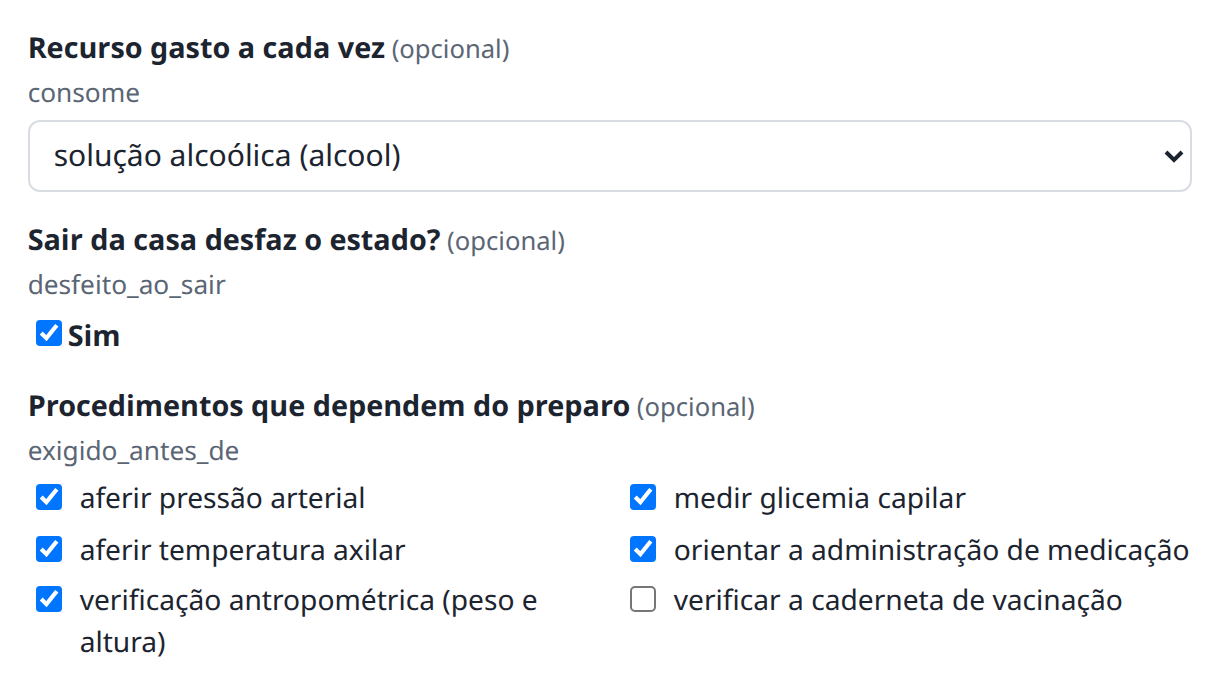
\includegraphics[width=6cm]{capturas/regras-formulario-trecho.png}};
  \node[exemplo,fill=blue!3] (e3) at (8.0,-.75) {\usebox{\pddl}};
  \node[exemplo,fill=blue!3] (e2) at (6.05,-2.95) {\usebox{\toml}};
  \node[exemplo,inner sep=0pt] (e4) at (11.4,-2.95)
    {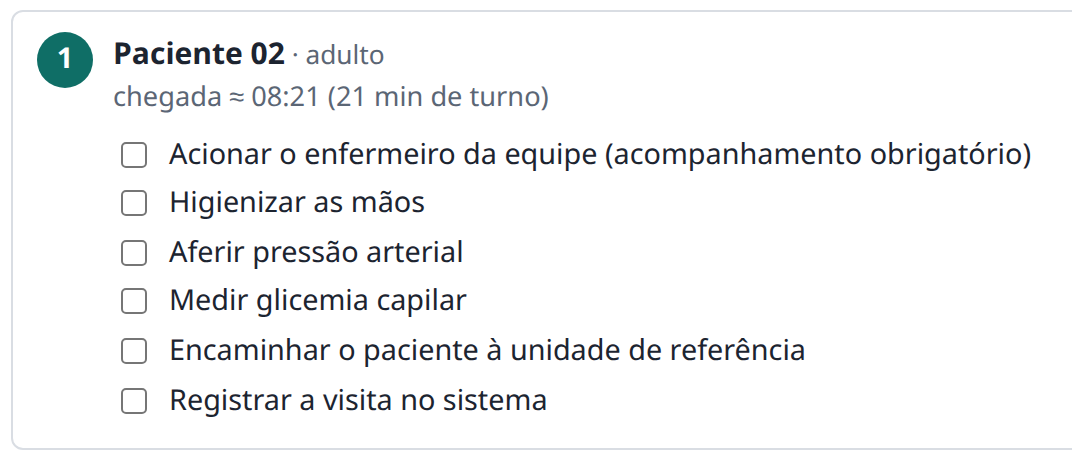
\includegraphics[width=6cm]{capturas/roteiro-visita.png}};
  \foreach \n in {1,...,4} \draw[liga] (n\n.south) -- (e\n.north);
\end{tikzpicture}
\end{document}
